% % $Id$

\chapter{Simulated Psychometric dataset}
\label{psychometric_dataset}
\minitoc

Before the invention of imaging techniques, the main methods used by neuroscientists were based on behavioral and physiological variables, such as, for example, psychometric tests and skin conductance responses.
\\

From PRoNTo v3.0, an important change was the possibility of analyzing these other types of data, as well as any other types of data, as long as they are transformed into .mat format according to some simple rules.
\\

This chapter will describe the steps necessary to perform classification and regression with a dataset with psychometric responses from a simulated dataset of a battery of psychometric tests in healthy controls and patients with depression. In reality, the main contribution of this chapter is to show users how to run an analysis with any general dataset in .mat files format.
\\

Since most of the topics have been covered already in the previous tutorials, the reader is advised to complete the previous tutorials before completing this one, because the explanation of some steps of this tutorial will be much less detailed. For the aforementioned reason, we will only include the GUI analysis.


\section{Classification}
\label{sec:psychometric_dataset_classification}


\subsection{Creating a general .mat dataset (optional)}
\label{ssec:psychometric_dataset_create_dataset}
In this section we will create a simulated psychometric dataset to classify healthy (\#190) versus depressed (\#190) individuals using three scales or questionnaires: negative affect scale (NA), anxiety scale (ANX) and an emotional regulation scale (ER). In this examples the different scales will represent different modalities and the different questions in each scale will represent different features (i.e. the files will contain an invididual scale question per column). The same scales will be used in regression later on to predict depression symptoms (DEP).

The files used in this chapter can be found in PRoNTo's website \url{http://www.mlnl.cs.ucl.ac.uk/pronto/prtdata.html}. In this link, the simulated psychometric datasets are already created so the this section is optional for the users that want to learn how to transform their data into the appropriate .mat file data format to be used to perform analyses within PRoNTo.
\\

We will start assuming we have our data in Excel sheets. In our case we have 2 groups (healthy controls and depressed patients) with 3 scales (ANX, ER and NA) per group, so we have 6 different excel sheets. Each row corresponds to a sample and each column corresponds to a feature/variable. In this case rows represent subjects, and columns represent the different scores in a test or different answers. When organizing the folder of your dataset it is good practice to have different folders for each group, and each modality (here our 3 psychometric scales), so we have created 2 folders with 3 subfolders each, to put our data in.

\begin{itemize}
    \item Starting from the ANX scale in depressed patients, we get inside the `ANX' subfolder, which is inside the `Depressed Patients' folder.
    \item We import the excel file named `ANX\_Dep.xlsx' in MATLAB as a numeric matrix. If done correctly, a 190x11 double precision matrix will appear in the MATLAB workspace. The default variable name with which the excel sheet will be imported in MATLAB will probably be `ANXDep'. 190 represents the number of depressed patients, and 11 represents the number of features in this modality.
    \item If you want, you can save the `ANXDep' matrix using the same name, making sure we are saving it in the correct folder. A new file named `ANXDep.mat' will appear.
    \item This matrix contains all 190 subjects in one matrix. As already mentioned in the manual, PRoNTo requires 1 file per subject, so we will use a script in the folder `utils' named `script\_create\_one\_file\_per\_row.m' to make that happen. Type `script\_create\_one\_file\_per\_row(ANXDep)'. As long as your matrix follows the aforementioned rules (rows = samples/subjects and columns = features) then the process should be successful and you will notice a new folder created with a default name `Samples\_mat', and inside it 190 files with a default name `Sample\_***.mat'.

\begin{itemize}
\item If you use your own scripts to create one file per subject, make sure that all of them have the same number of characters. If for example you have 10 subjects, the first 9 subjects should have the name `name\_01.mat' to `name\_09.mat', so that they have the same number of characters with `name\_10.mat', otherwise PRoNTo will throw an error. They \textbf{should not} be named `name\_1.mat' to `name\_9.mat' and `name\_10.mat'.
\end{itemize}

\end{itemize}

Repeat the same procedure for all the other modalities and groups.

\subsection{GUI analysis}

To start, create a new folder in which to save the results of the analysis, then start up MATLAB and type `prt' or `pronto' in the MATLAB prompt. This will open the main interface of PRoNTo.


\subsection{Data \& Design}

\begin{itemize}
	
	\item In PRoNTo's main window, click on `Data \& Design'. Like in the previous chapters, browse the folder in which to save the PRT structure (saved as `PRT.mat');
	
	\item In the panel `Groups', click on `Add' and provide a name for the groups, with no spaces, in our case `DEP'.
	
	\item In the panel `Subjects/Samples', click on the `Samples' tick box below the panel.
	
	\item In the `Modalities' panel:
	
	\begin{itemize}
	\item Click on `Add' and provide a name to the modality, e.g. `ANX'. \item In the `Data format', choose `.mat'.
	\item Load all the files available in the `ANX' folder (dataset\_psychometric/Classification/Depressed Patients/ANX). You can select all the files by using the right mouse button and clicking on the option `Select All'. When all the files are selected, click on the `Done' button.
	
	\item Leave the `Regression targets' and `Covariates' section as they are, and press `OK'.
	\end{itemize}
	
	Repeat the same procedure for all 3 modalities and 2 groups.
	
	\item Leave the `Masks field as it is.

	\item Click on the 'Save' button to create the `PRT.mat' file with the structure containing the information that has been previously specified. If no errors are shown in the MATLAB command, leave the `Data and design' window by clicking `Quit'.
	
\end{itemize}

The `Data and design' window should look similar to the one in Figure \ref{fig:psychometric_dataset_gui_data_and_design_final}.

		\begin{figure}[!h]
	\centering
		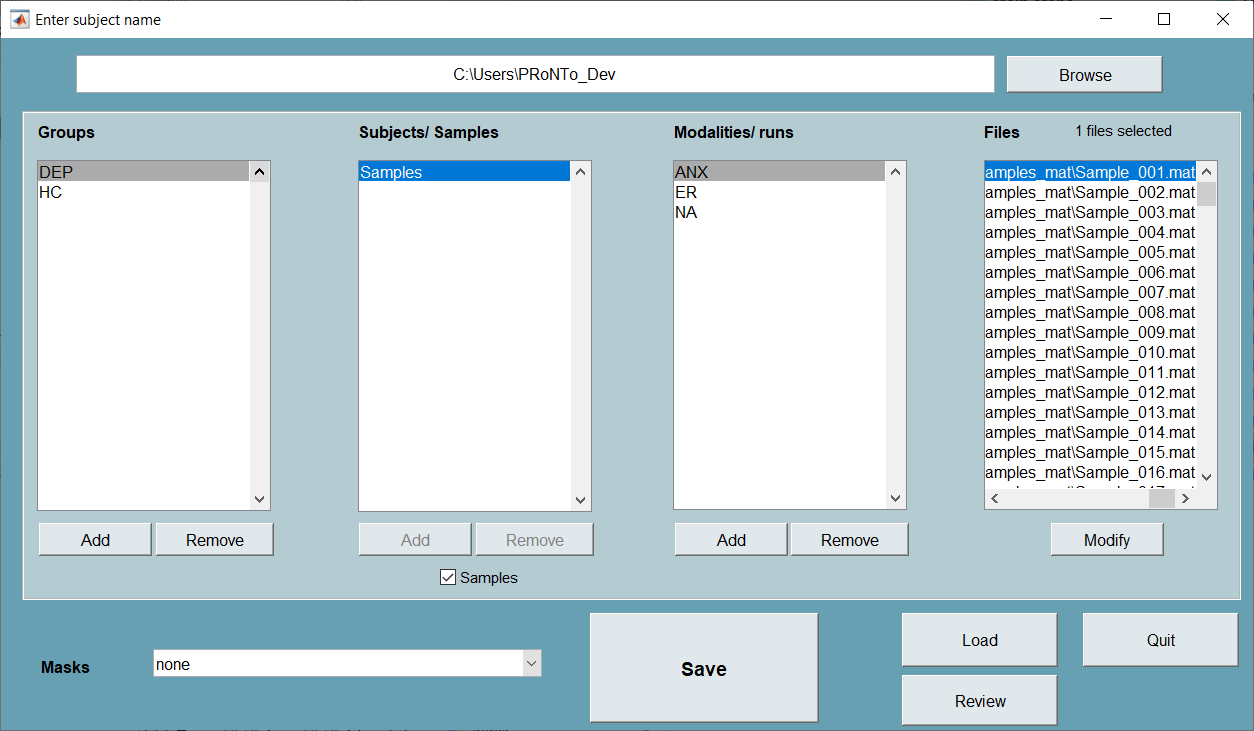
\includegraphics[scale=0.6]{images/Tutorial/v3/psychometric_dataset/psychometric_dataset_gui_data_and_design_final.png}
	\caption{`Data and design' GUI final configuration.}
	\label{fig:psychometric_dataset_gui_data_and_design_final}
\end{figure}

% %--------------------------------------------------------

\subsection{Prepare feature set}

\begin{itemize}
	
	\item Next we have to prepare the feature set, so click on `Prepare feature set' in PRoNTo's main window. A new window will open prompting you to select a PRT.mat file. Select the `PRT.mat' file previously created in the `Data \& Design' step, as in Figure \ref{fig:gui_prepare_featureSet_choose_PRT} from Chapter \ref{sec:Block_design_fMRI_dataset}.
	
	\item Once you click `Done' another window will appear, `Prepare feature set'. Type a name for your feature set, e.g. `ANX' and choose how many sessions you want to concatenate, in our case 1.
	
	\item Once you type the number of sessions yet another window will appear, `Specify modality to include'. Here you set the specification of different parameters and options for each modality. In our case you only have to select the `ANX' modality you previously specified in the `Data \& Design' step.
	
	\item Finally, click on the 'Done' button, and then the `Build kernel / data matrix' button.

\end{itemize}

After you are finished with the ANX modality, repeat the procedure for the other two modalities, ER and NA.

	\begin{figure}[!h]
	\centering
		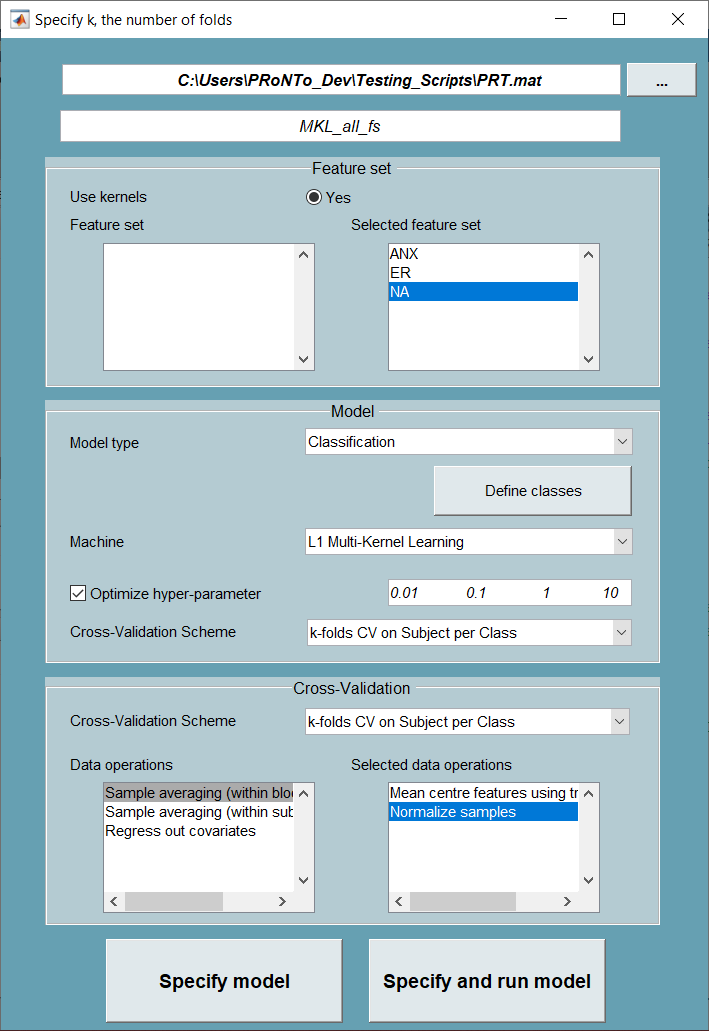
\includegraphics[width=0.5\textwidth]{images/Tutorial/v3/psychometric_dataset/psychometric_dataset_gui_specify_model_new_final.png}
	\caption{`Specify model new' GUI final configuration.}
	\label{fig:psychometric_dataset_gui_specify_model_new_final}
\end{figure}

% %---------------------------------------------------------------------

\subsection{Model: Specify new}

\begin{itemize}
	
	\item In PRoNTo's main window, click on `Specify model' and a new window called `Specify model' will open (see Figure \ref{fig:gui_specify_new} in Chapter \ref{sec:Block_design_fMRI_dataset});
	
	\item Select the `PRT.mat' file and provide a name to the model, e.g. `MKL\_all\_fs';

	\item Select all 3 feature sets previously defined;

	\item Leave the option `Use kernels' tick box as it is, i.e. `Yes'. This step is optional and depends on the choice of model;

	\item	Select the `Classification' model type and click on the 'Define classes` button. A new window will open, `Specify classes', to define the number of classes and the name for each class. We will define 2 classes. First click `Class 1' on the tab `Class'. `Class 1' will be all the depressed patients, so select the `DEP' group and then select all subjects. Similarly for `Class 2' select all subjects in the `HC' group. Leave the `Subsample according to smallest class' as it is for now. Once you have appropriately specified everything, click `Done';
	
	\item Select the `L1 Multi-Kernel Learning' option, in the `Machine' field;
	
	\item Select the `Optimize hyper-parameter' tick box, leave the `Define Range' at its default range (i.e. [0.01 0.1, 1, 10, 100, 1000]) and in the `Cross-Validation Scheme' (internal loop) field, select the option `k-fold CV on Subjects per Class'. A window will appear asking to define the value of k, set it to 5.
		
	\item Select the `k-fold CV on Subjects per Class' cross-validation scheme (external loop), again with k=5; 
	
	\item In the `Data operations' box, select the `Mean centre features using training data' and `Normalize samples' options Then, the `Specify model' window should look similar to the one in Figure \ref{fig:psychometric_dataset_gui_specify_model_new_final};
	
	\item Click on `Specify and run model' and the model will be immediately estimated, therefore there is no need to use the `Run model' module in this case. If however you wanted to check the statistical significance of your results, you need to use the `Run model' module in order to do permutation testing. It will take a few minutes to complete.

\end{itemize}

The MKL machine will learns the contribution of each scale (scales or kernel weights) and the contribution of each question within each scale (questions weights) to build the prediction function.
\\

For this dataset, it could be useful to also run the analysis with a non-kernel method, like L1-SVM. Just repeat the steps as described above, unclick the “Use Kernel” option, choose the ‘Binary L1-SVM’ machine and do not include the ‘Normalize samples’ data operation.




% \begin{figure}[!h]
% 	\centering
% 	\begin{minipage}[b][13cm][b]{0.5\textwidth}
%   \centering
% 		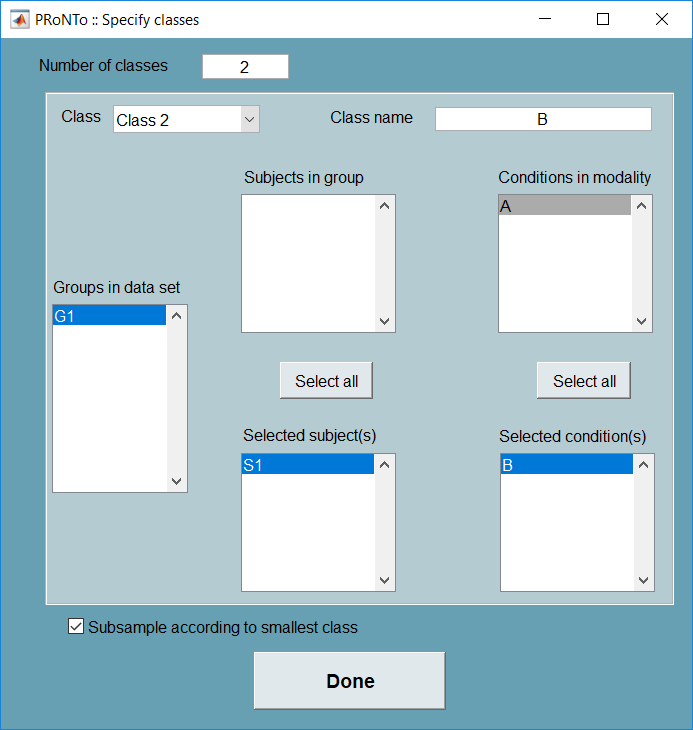
\includegraphics[scale=0.55]{images/Tutorial/v3/semi_simulated_ecog/ecog_gui_specify_model_specify_classes.png}
% 		  \captionsetup{width=0.9\linewidth}
% 	\captionof{figure}{`Specify classes' GUI.}
% 	\label{fig:ecog_gui_specify_model_specify_classes}
% \end{minipage}%
% 	\begin{minipage}[b][13cm][b]{0.5\textwidth}
%   \centering
% 		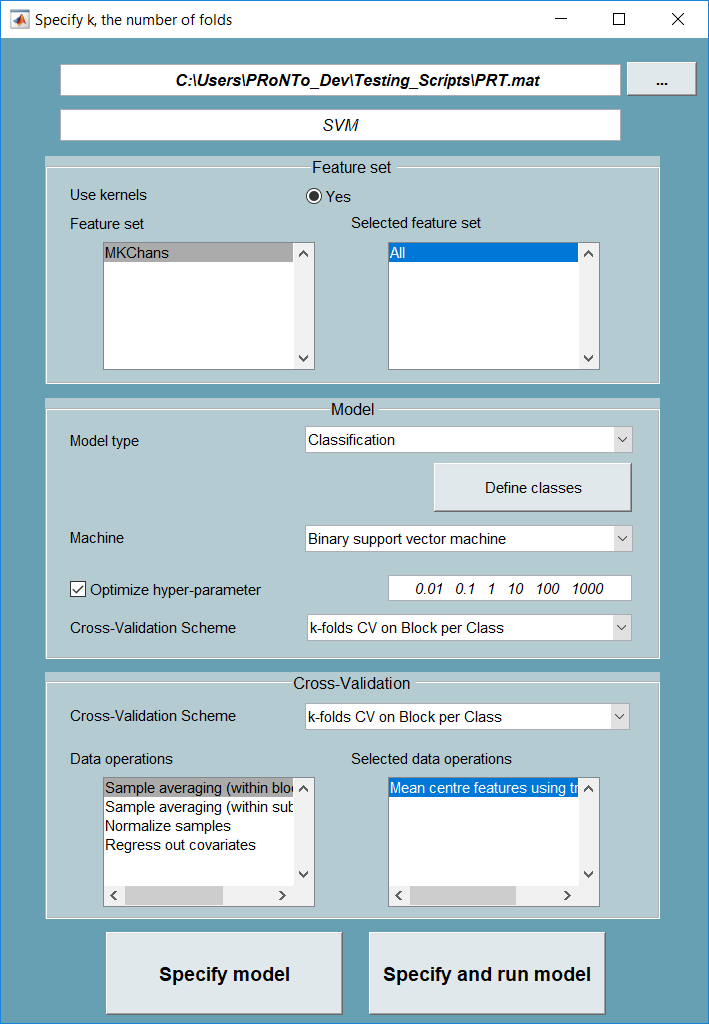
\includegraphics[scale=0.55]{images/Tutorial/v3/semi_simulated_ecog/ecog_gui_specify_model_svm_final.png}
% 		\captionsetup{width=0.9\linewidth}
% 	\captionof{figure}{`Specify model' GUI, `SVM' model.}
% 	\label{fig:ecog_gui_specify_model_svm_final}
% 	\end{minipage}
% \end{figure}









% %--------------------------------------------------------------------

\subsection{Display results}
\label{psychometric_dataset_class_display_results}

In PRoNTo's main window, click on `Display results' and select the `PRT.mat' file. This will open the main results window. In the `Model' panel, select the model that you want to view, `MKL\_all\_fs', and the results through performance will be similar to the one in Figure \ref{fig:psychometric_dataset_gui_display_results}. Also keep in mind that if you have not run permutation tests, all p-values would be `N.A.'.

		\begin{figure}[!h]
	\centering
		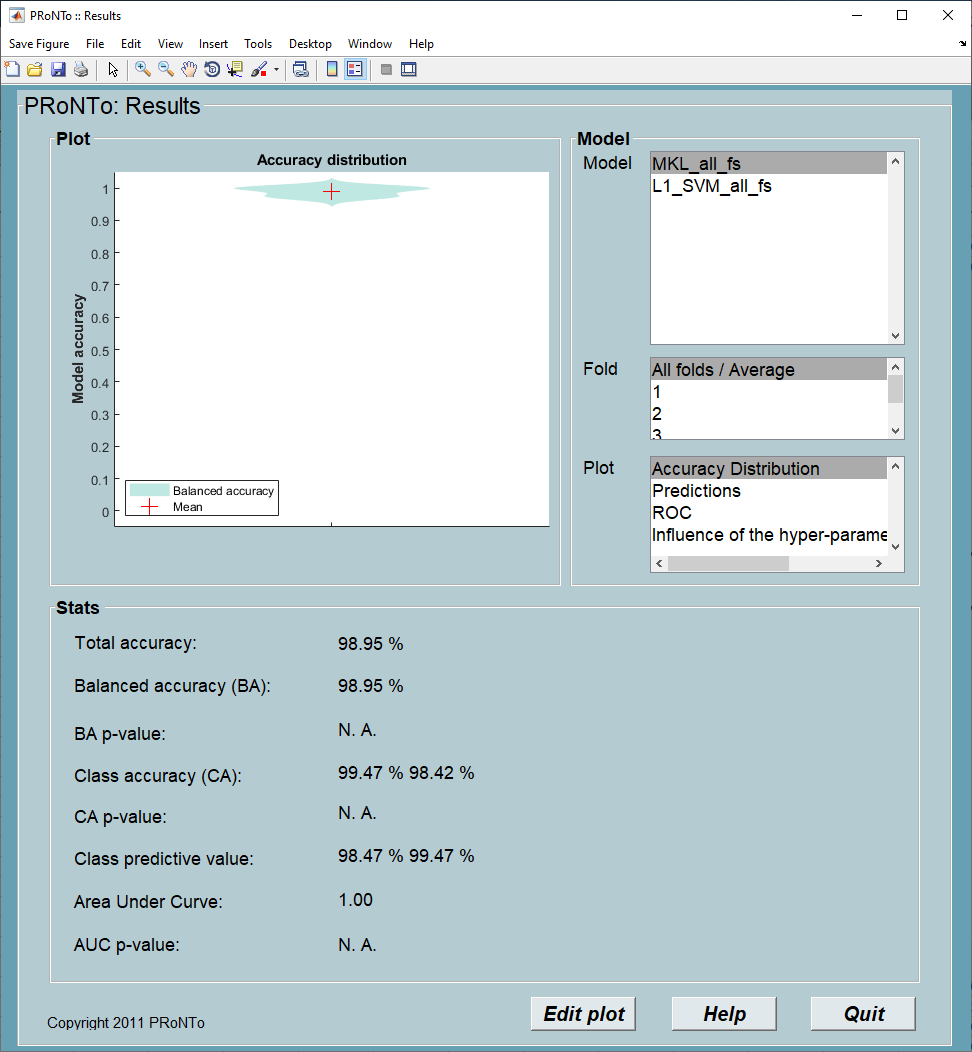
\includegraphics[width=0.6\textwidth]{images/Tutorial/v3/psychometric_dataset/psychometric_dataset_gui_display_results.png}
	\caption{`Display results' GUI.}
	\label{fig:psychometric_dataset_gui_display_results}
\end{figure}


% %------------------------------------------------------------------

\subsection{Compute and Display weights}

\begin{itemize}
\item In PRoNTo's main window, click on `Compute weights' and a new window will open, `Compute weights' (see Figure \ref{fig:gui_compute_weights} in Chapter \ref{sec:Block_design_fMRI_dataset}); 

\item Select the `PRT.mat' file;

\item In the drop-down list `Models computed in PRT', select the `MKL\_all\_fs' model;

\item And finally click the button `Compute weights'.

\end{itemize}

After you finish computing the weights and clicking on the `Display weights' module the weight contributions for the ANX modality and the weights for the different feature sets (ER, NA, ANX) should look similar to the ones in Figure \ref{fig:psychometric_dataset_gui_display_weights};

\begin{figure}[!h]
	\centering
		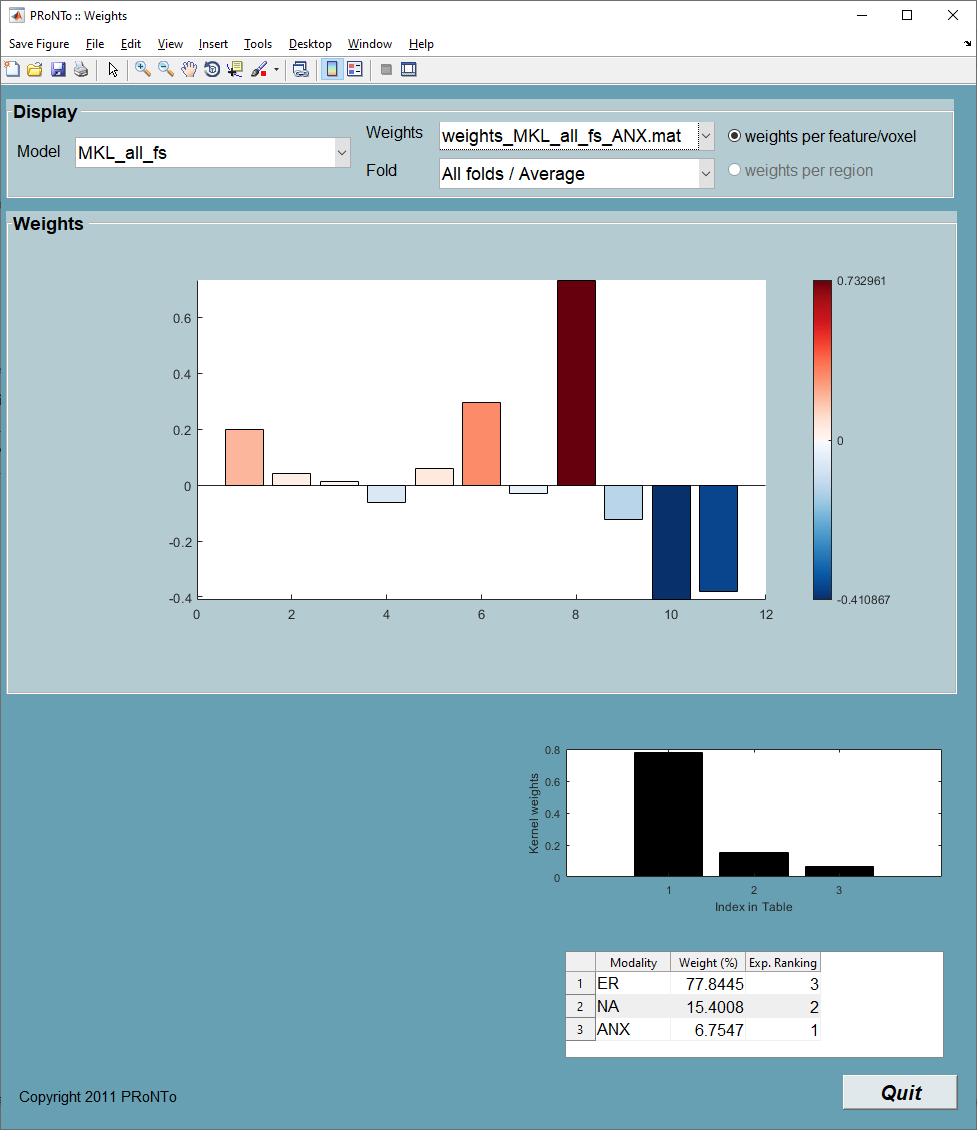
\includegraphics[width=0.6\textwidth]{images/Tutorial/v3/psychometric_dataset/psychometric_dataset_gui_display_weights.png}
	\caption{`Display weights' GUI.}
	\label{fig:psychometric_dataset_gui_display_weights}
\end{figure}

% %=====================================================



% %=====================================================

\section{Regression}

In this section we will again use similar groups and features as in section \ref{sec:psychometric_dataset_classification}. Whereas in the previous section the aim of the analysis was to classify depressed from healthy individuals, in this section our aim is to try to predict the depression score of different individuals.

\subsection{Creating a general .mat dataset (optional)}

First the user should follow the steps in \ref{ssec:psychometric_dataset_create_dataset} in order to create the data to use for the regression example. Make sure to use the excel sheets inside the `Regression' folder
\\

In regression, we also have to define a regression target. In our case here we are trying to predict the "score" in depression symptoms. The values of the depression symptoms scores for our subjects are in the excels titled `RT\_DEP.xlsx' and `RT\_HC.xlsx'.
\\

As mentioned earlier in the manual, from PRoNTo v3.0 the user can include multiple regression targets. The rows represent the samples (in our case the number of subjects, 190), and each column represents one regression target. So in our case we will have a 1-column vector of length 190 for each group. The name of this column or matrix \textbf{must be} `rt\_subj'.
\\

PRoNTo also requires the names of the regression targets in a cell array, where as in `rt\_subj' also, each column represents one regression target. Let's name our regression target `DEP'. The name of this row vector \textbf{must be} `names'.
\\

So after we build the data, the user should import the excel in MATLAB for the regression targets too. More specifically:

\begin{itemize}
    \item After you import `RT\_DEP.xlsx', rename it to `rt\_subj' which is the name required by PRoNTo.
    
    \item We also have to create the `names' array. For that, type `names = {'DEP'};'  in the MATLAB command window.
    
    \item Finally, type `save('RT\_DEP.mat','rt\_subj','names');' in order to save the file with its two arrays, while making sure you are inside the `Depression Patients' folder.
    
\end{itemize}

Repeat the same procedure for the `Healthy Controls'.

\subsection{GUI analysis}

To start, create a new folder in which to save the results of the analysis, then start up MATLAB and type `prt' or `pronto' in the MATLAB prompt. This will open the main interface of PRoNTo.


\subsection{Data \& Design}

This module is going to follow the same steps as in the previous section, \ref{sec:psychometric_dataset_classification}.

\begin{itemize}
	
	\item In PRoNTo's main window, click on `Data \& Design'. Like in the previous chapters, browse the folder in which to save the PRT structure (saved as `PRT.mat');
	
	\item In the panel `Groups', click on `Add' and provide a name for the groups, with no spaces, in our case `DEP'.
	
	\item In the panel `Subjects/Samples', click on the `Samples' tick box below the panel.
	
	\item In the `Modalities' panel:
	
	\begin{itemize}
	\item Click on `Add' and provide a name to the modality, e.g. `ANX'. \item In the `Data format', choose `.mat'.
	\item Load all the files available in the `ANX' folder (dataset\_psychometric/Regression/Depressed Patients/ANX). You can select all the files by using the right mouse button and clicking on the option `Select All'. When all the files are selected, click on the `Done' button.
	
	\item In the `Regression targets' field select `Specify targets'. A new window will appear, `Specify targets'. In the `Targets' section select `From a .mat file' and select the `RT\_DEP.mat' file that we created. After selecting the file your window should look similar to the one in Figure \ref{fig:psychometric_dataset_gui_data_and_design_specify_targets}.

		\begin{figure}[!h]
	\centering
		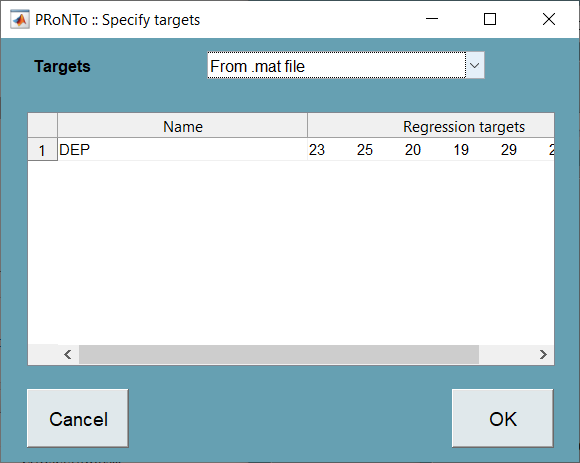
\includegraphics[scale=0.6]{images/Tutorial/v3/psychometric_dataset/psychometric_dataset_gui_data_and_design_specify_targets.png}
	\caption{`Specify targets' GUI configuration for Depressed Patients.}
	\label{fig:psychometric_dataset_gui_data_and_design_specify_targets}
\end{figure}
	
	\item Leave the `Covariates' section as it is, and press `OK'.
	\end{itemize}
	
	Repeat the same procedure for all 3 modalities and 2 groups.
	
	\item Leave the `Masks' field as it is.

	\item Click on the 'Save' button to create the `PRT.mat' file with the structure containing the information that has been previously specified. If no errors are shown in the MATLAB command, leave the `Data and design' window by clicking `Quit'.
	
\end{itemize}

The `Data and design' window should look similar to the one in Figure \ref{fig:psychometric_dataset_gui_data_and_design_final}, which is the same as in classification, with the only difference that now we have also included regression targets in our modalities.

% %--------------------------------------------------------

\subsection{Prepare feature set}

This module is exactly the same as in section \ref{sec:psychometric_dataset_classification}.

\begin{itemize}
	
	\item Click on `Prepare feature set' in PRoNTo's main window. A new window will open prompting you to select a PRT.mat file. Select the `PRT.mat' file previously created in the `Data \& Design' step, as in Figure \ref{fig:gui_prepare_featureSet_choose_PRT} from Chapter \ref{sec:Block_design_fMRI_dataset}.
	
	\item Once you click `Done' another window will appear, `Prepare feature set'. Type a name for your feature set, e.g. `ANX' and choose how many sessions you want to concatenate, in our case 1.
	
	\item Once you type the number of sessions yet another window will appear, `Specify modality to include'. Here you set the specification of different parameters and options for each modality. In our case you only have to select the `ANX' modality you previously specified in the `Data \& Design' step.
	
	\item Finally, click on the 'Done' button, and then the `Build kernel / data matrix' button.

\end{itemize}

After you are finished with the ANX modality, repeat the procedure for the other two modalities, ER and NA.

% %---------------------------------------------------------------------

\subsection{Model: Specify new}

Most differences will be in this module.


\begin{itemize}
	
	\item In PRoNTo's main window, click on `Specify model' and a new window called `Specify model' will open (see Figure \ref{fig:gui_specify_new} in Chapter \ref{sec:Block_design_fMRI_dataset});
	
	\item Select the `PRT.mat' file and provide a name to the model, e.g. `eSVR\_all\_fs\_K5';

	\item Select all 3 feature sets previously defined;

	\item Unclick the option `Use kernels' tick box, i.e. `No';

	\item	Select the `Regression' model type and click on the `Select subjects/scans' button. A new window will open, `Specify subjects/targets for regression'. Select all subjects from the DEP group, as well as our regression target, `DEP';
	
	\item Select the `epsilon-SVR' option, in the `Machine' field;
	
	\item Select the `Optimize hyper-parameter' tick box, leave the `Define Range' at its default range (i.e. [0.01, 0.1, 1, 10, 100, 1000]) and in the `Cross-Validation Scheme' (internal loop) field, select the option `k-fold CV on Subject Out'. A window will appear asking to define the value of k, set it to 5.
		
	\item Select the `k-fold CV on Subject Out' cross-validation scheme (external loop), again with k=5; 
	
	\item In the `Data operations' box, select the `Mean centre features using training data'. Then, the `Specify model' window should look similar to the one in Figure \ref{fig:psychometric_dataset_gui_regression_specify_model_new_final};
	
	\begin{figure}[!h]
	\centering
		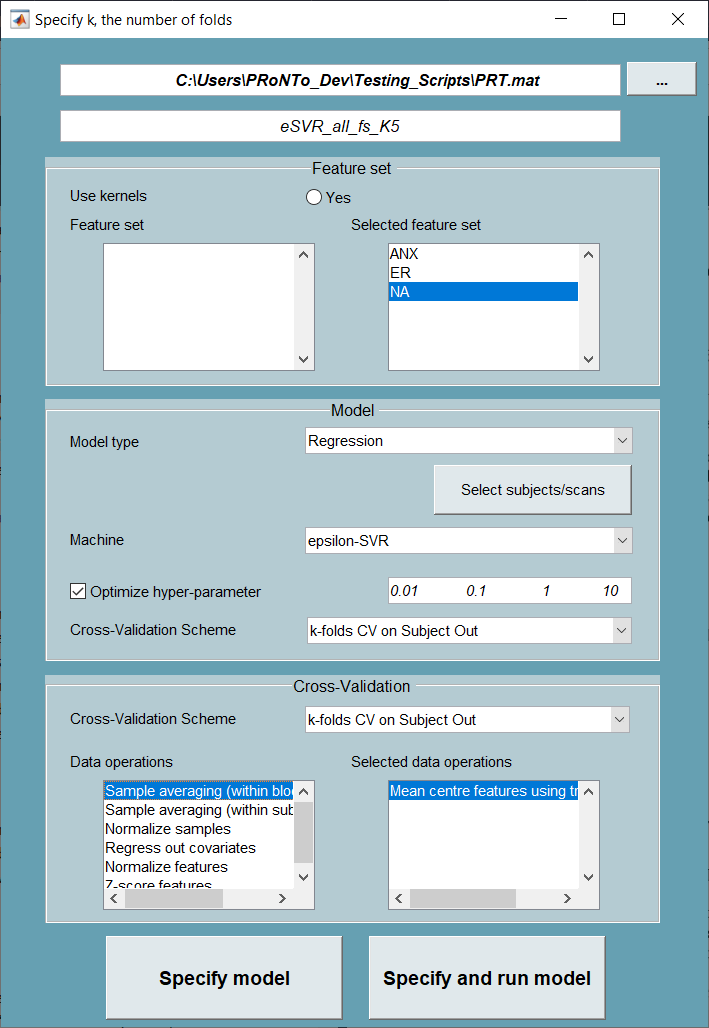
\includegraphics[width=0.5\textwidth]{images/Tutorial/v3/psychometric_dataset/psychometric_dataset_gui_regression_specify_model_new_final.png}
	\caption{`Specify model new' GUI final configuration for regression.}
	\label{fig:psychometric_dataset_gui_regression_specify_model_new_final}
\end{figure}
	
	\item Click on `Specify and run model' and the model will be immediately estimated, therefore there is no need to use the `Run model' module in this case. If however you wanted to check the statistical significance of your results, you need to use the `Run model' module in order to do permutation testing. It will take a few minutes to complete.

\end{itemize}

For this dataset, it could be useful to also run the analysis with a multiple kernel method, like MKL so that we also learn the weight contribution of each feature set or modality independently. Just repeat the steps as described above, click the “Use Kernel” option, choose the MKL machine and include the ‘Normalize samples’ data operation.


% %--------------------------------------------------------------------

\subsection{Display results}
\label{psychometric_dataset_regression_display_results}

In PRoNTo's main window, click on `Display results' and select the `PRT.mat' file. This will open the main results window. In the `Model' panel, select the model that you want to view, `eSVR\_all\_fs\_K5', and the results plot through performance will be similar to the one in Figure \ref{fig:psychometric_dataset_gui_regression_display_results}. Also keep in mind that if you have not run permutation tests, all p-values would be `N.A.'.
	
	\begin{figure}[!h]
	\centering
		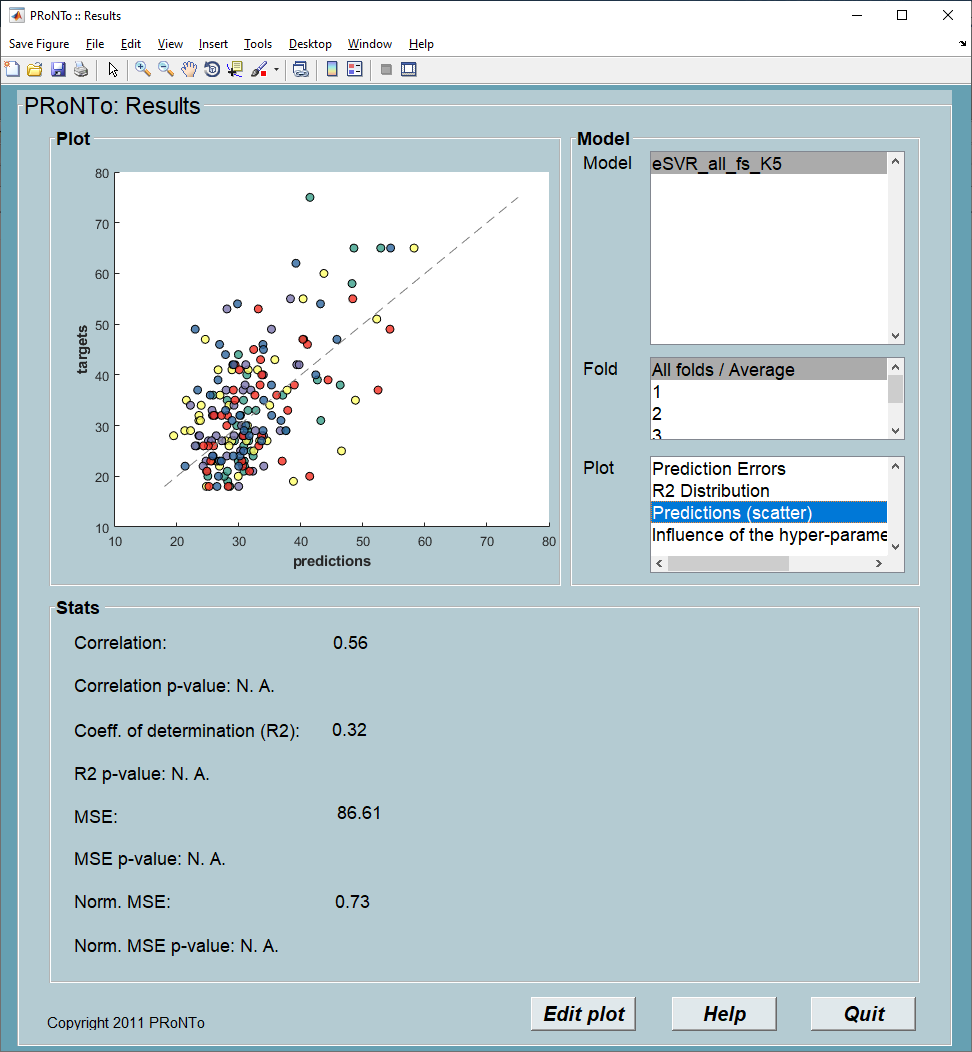
\includegraphics[width=0.57\textwidth]{images/Tutorial/v3/psychometric_dataset/psychometric_dataset_gui_regression_display_results.png}
	\caption{`Display results' GUI.}
	\label{fig:psychometric_dataset_gui_regression_display_results}
\end{figure}
	

		
	
% %------------------------------------------------------------------

\subsection{Compute and Display weights}

In PRoNTo's main window, click on `Compute weights' and a new window will open, `Compute weights' (see Figure \ref{fig:gui_compute_weights} in Chapter \ref{sec:Block_design_fMRI_dataset}). After select the `PRT.mat' file, in the drop-down list `Models computed in PRT', select the `eSVR\_all\_fs\_K5' model, and finally click the button `Compute weights'.
\\

After you finish computing the weights and clicking on the `Display weights' module the weight contributions for the ER feature set should look similar to the ones in Figure \ref{fig:psychometric_dataset_gui_regression_display_weights}. In a similar way, you will be able to see the weight contribution for the other modalities (ANX and NA).

\begin{figure}[!h]
	\centering
		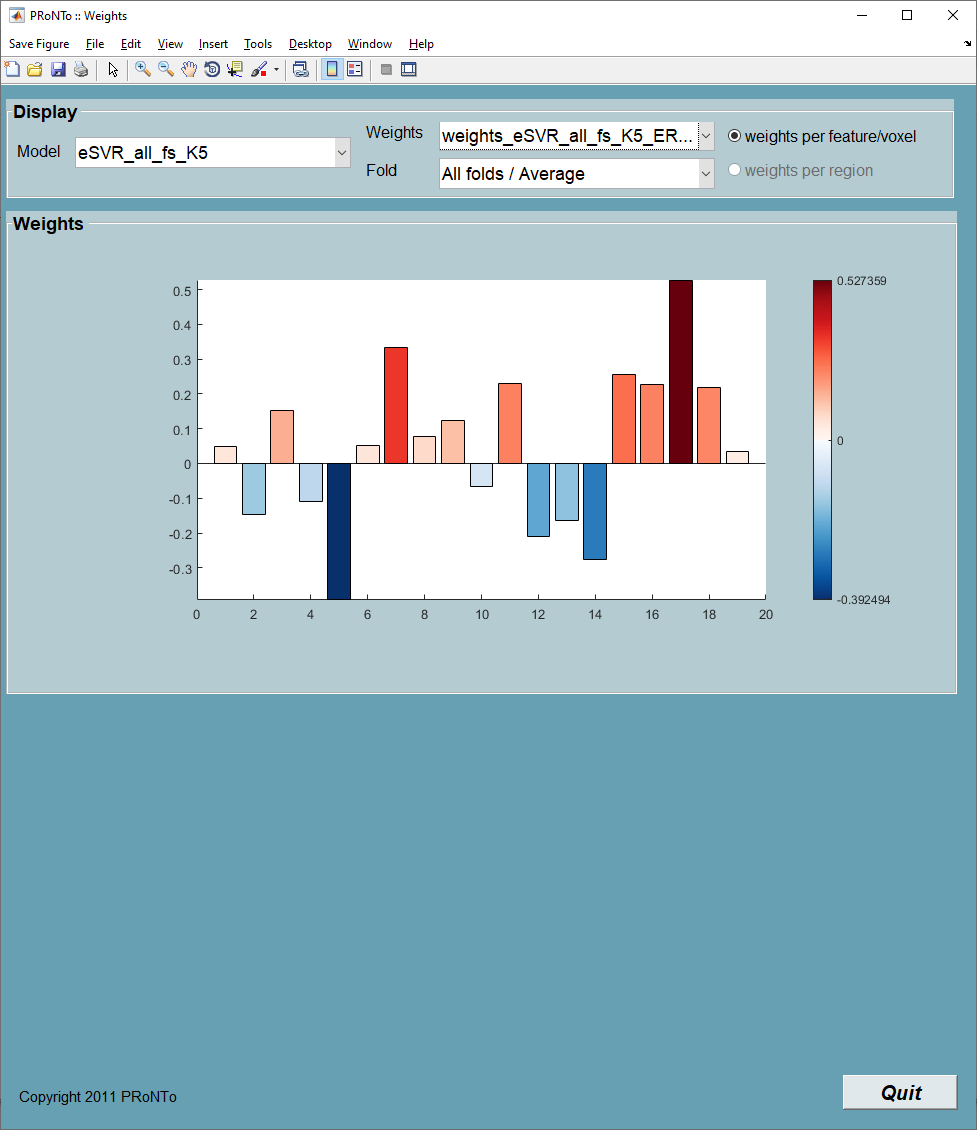
\includegraphics[width=0.55\textwidth]{images/Tutorial/v3/psychometric_dataset/psychometric_dataset_gui_regression_display_weights.png}
	\caption{`Display weights' GUI.}
	\label{fig:psychometric_dataset_gui_regression_display_weights}
\end{figure}
	








